% This is samplepaper.tex, a sample chapter demonstrating the
% LLNCS macro package for Springer Computer Science proceedings;
% Version 2.20 of 2017/10/04
%
\documentclass[runningheads]{llncs}
%
\usepackage{graphicx}
\usepackage{cite}
\usepackage{amsmath}
% Used for displaying a sample figure. If possible, figure files should
% be included in EPS format.
%
% If you use the hyperref package, please uncomment the following line
% to display URLs in blue roman font according to Springer's eBook style:
% \renewcommand\UrlFont{\color{blue}\rmfamily}

\begin{document}
%
\title{Rule Driven Query Expansion}
%
%\titlerunning{Abbreviated paper title}
% If the paper title is too long for the running head, you can set
% an abbreviated paper title here
%
% \author{Xinze Lyu,
% Wei Hu \and Yuzhong Qu}
%
\authorrunning{F. Author et al.}
% First names are abbreviated in the running head.
% If there are more than two authors, 'et al.' is used.
%
% \institute{State Key Laboratory for Novel Software Technology, Nanjing University, China \and
% Department of Computer Science and Technology, Nanjing University, China
% \email{xzlv.nju@gmail.com, {whu,yzqu}@nju.edu.cn}\\
% }
%
\maketitle              % typeset the header of the contribution
%
\begin{abstract}
  Empty answers problem exists when we use SPARQL to access RDF knowledge graph data. Put situations that querying facts inexistent to the real world aside, one reason is that users lack enough knowledge for a particular RDF knowledge graph, that leads to SPARQL queries with wrong formats or inaccurate expressions.  However, due to the schema-free nature of RDF data and incompleteness of particular RDF knowledge graphs, even a SPARQL query with correct format can reflect users' intentions accurately, it may fail to get any results. Researches going on in translating the natural language to SPARQL help a lot to address the first problem, but these are inconducive for the second problem which was caused by the faults in structure and content of RDF knowledge graphs.
  We design a rule-driven framework to alleviate the obstacles caused by the structure and content of RDF knowledge graphs. Specifically, given a SPARQL query, we use knowledge graph oriented rule-learning procedure to take reasoning rules, with the help of these rules, our system return possible results. More importantly, our system shows detailed information with similarity score and rules to explain why our system chooses particular possible answers.
\keywords{SPARQL  \and Empty Answer \and Rule Learning.}
\end{abstract}
%
%
%
\section{Problem Statement}
\subsection{Empty Answer Problem for SPARQL query}
Users use SPARQL queries reflecting their intentions to access the  data from RDF knowledge graph, reasons for Empty Answer Problem are various, three of which are main ones: 1) the facts that users want to query do not exist in the real world, this may be caused by the wrong mapping of entities or relations, the misplace of subjects or objects; 2) the formats of SPARQL is wrong, including  the namespace, operators and so on; 3) SPARQL queries are accurate and well-formatted, but they do not have exact matches in particular RDF knowledge graphs.

The problem 1) and 2) can be regarded as users can not use SPARQL language descripe their intentions, there are lots of works being done to solve this problem, including entity linking~\cite{el_Han}, relation linking~\cite{dubey2018earl} and more sophisticated work, translating natural language into SPARQL~\cite{sander2014ontology}.
These works are done under the situation that users lack the full knowledge of particular RDF knowledge graph, they aim to help users to generate well-formatted SPARQL query to reflect their intentions accurately, however, it is not enough. Even a SPARQL query can avoid the problem 1) and 2), it may still has to face problem 3).
For example, when a user want to know \textit{``Who is the advisor of Newton?"}, he makes a SPARQL in table~\ref{Newton} to access Dbpedia, this is a correct SPARQL query, but it gets no answer because there is not an entity that exists explicit relation \textit{``dbo:doctoralAdvisor"} with \textit{``dbr:Isaac\_Newton"}. But Newton really has advisors, it is \textit{``dbr:Isaac\_Barrow"}, this fact is recorded as \textit{``dbr:Isaac\_Newton dbo:academicAdvisor dbr:Isaac\_Barrow" } in Dbpeida.  This seems that we can make some ``magic operations" to link word ``advisor" to \textit{``dbo:academicAdvisor"} instead of \textit{``dbo:doctoralAdvisor"}, we also prepare another example in table~\ref{film_table}. We construct this query to get Asian directors and their films. It gets no answer, too. Although some directors' birthplaces are connected to \textit{``dbr:China"}, \textit{``dbr:Japan"} and so on, they are Asian directors absolutely, but no one's birthplace is connected to \textit{``dbr:Asia"} directly.

\begin{table}
\caption{SPARQL to get Asian films and their films.}\label{film_table}
\centering
\begin{tabular}{|c|lll|}
\hline
\multicolumn{4}{|l|}{SELECT ?film ?director WHERE }\\
\hline
(1) &  ?film & dbo:director & ?director.\\
(2) &  ?director & dbo:birthPlace & dbr:Asia.\\
\hline
\end{tabular}
\end{table}

In this paper, we assume that our SPARQL queries are not related to problem 1) and 2) and focus on problem 3).
Problem 1) and 2) are more related to Natural Language Processing, Problem 3) is different, it is caused by the inherent limits(or features) of RDF knowledge graph. RDF knowledge graph is schema-free, there are often several similar predicates to describe the same relation, this leads to the problem about ``Newton's advisors" above; RDF knowledge graph is incomplete, it is also impossible to make a single complete RDF knowledge graph now, so it leads to the problem about ``Asian" presented above.

More clearly, Problem 3) has 2 typical kinds of expressions.
One is the SPARQL queries have a high level of constraints, we get an instance from the released resource of~\cite{wangEmbed}, there are three constraints for the SPARQL query in table~\ref{Over_C_Example}. This query gets no answers, in fact, the constraints (1) and (2) are redundant, we can infer that ``?company" is ``dbr:Apple\_Inc" only with constraints (3). It seems good to relax or delete the unnecessary constraints. Some works tried to solve it by Query Relaxation techniques, including replacement with similar entities and predicates~\cite{elbassuoni2011query}, relaxation with ontology rule~\cite{2010combining} and approximation for related results with representation learning in vector space~\cite{wangEmbed, hamilton2018embedding, zhang2018trquery}. Some works try to find which parts of a SPARQL query should be deleted, but it is a NP-hard problem and do not get good results. Also, there are works ~\cite{huang2012} that try to construct this problem as a complete document IR problem, which needs extra text sources. We will detail these methods later.

Besides high level constraints query, there are many simple and plain SPARQL queries, like SPARL in table~\ref{Newton}, relaxation techniques are not proper for these simple queries, because relaxation will change the meaning of simple SPARQL queries easily.

\begin{table}
\caption{SPARQL with high constraints.}\label{Over_C_Example}
\centering
\begin{tabular}{|c|lll|}
\hline
\multicolumn{4}{|l|}{SELECT ?company WHERE }\\
\hline
(1) &  ?company & rdfs:type & dbo:Company.\\
(2) &  ?company  & dbo:industry  & dbr:Electronics.\\
(3) & dbr:IPhone & dbp:developer & ?company.\\
\hline
\end{tabular}
\end{table}

\begin{table}
\caption{SPARQL to get the advisors of Newton.}\label{Newton}
\centering
\begin{tabular}{|c|lll|}
\hline
\multicolumn{4}{|l|}{SELECT ?advisor WHERE }\\
\hline
(1) &  dbr:Isaac\_Netwon & dbo:doctoralAdvisor & ?advisor.\\
\hline
\end{tabular}
\end{table}
% \subsubsection{Sample Heading (Third Level)}
% \paragraph{Sample Heading (Fourth Level)}
\subsection{Semantic Parsing}
\subsection{Paraphrasing}
\subsection{Similarity Based Method}
The idea behind similarity based method is straight and simple, it wants to replace certain entities or relations with similar ones to get approximated results. For SPARQL in table~\ref{film_table}, replacing \textit{``dbr:Electronics"} with its similar one \textit{``dbr:Computer\_hardware"} will make this SPARQL return \textit{``dbr:Apple\_Inc"} successfully.

This kind of works~\cite{elbassuoni2011query} are often constructed by two stages: 1)design approaches to calculate the similarity between entities and relations; 2)design stategies to replace entities and relations in original SPARQL queries.

We want to point out 2 drawbacks of this method.
\begin{enumerate}
  \item It is hard to definen ``similar". Take SPARQL in table~\ref{Netwon_s_t} for example, users want to query Newton's students and advisors. For the first constraint, if we want to try to replace entity \textit{``dbr:Isaac\_Newton"}, we should choose Newton's classmates; for the second constraints, Newton's colleagues are more better. Similarity resides in aspects. Similar entites should be choosen according to the situations, but existing methods just choose entites under a fixed similarity ranking.
  \item To our best of knowledge, existing entities similarity or relatedness methods~\cite{ponza2017two,2014deepwalk} often neglect the influence of predicates, they regard RDF knowledge graph as social networks to calculate similarity between entites. Triples relatedness~\cite{2018weakly} may be a good direction to get high quality and fine-grained entities relatedness. Predicates similarity or relatedness is rarely studied.
\end{enumerate}

\begin{table}
\caption{SPARQL to get the advisors and students of Newton.}\label{Netwon_s_t}
\centering
\begin{tabular}{|c|lll|}
\hline
\multicolumn{4}{|l|}{SELECT ?advisor ?student WHERE }\\
\hline
(1) &  dbr:Isaac\_Netwon & dbo:doctoralAdvisor & ?advisor.\\
(2) & ?student & dbo:doctoralAdvisor & dbr:Isaac\_Netwon.\\
\hline
\end{tabular}
\end{table}

\subsection{Ontology Rule Based Method}
This kind of method~\cite{2010combining} follows rules in table ~\ref{RDFS_rules}. Given an ontology $K$, this method computes the \textit{extended reduction} $extRed(K)$ of $K$ as follows: (i) compute the closure of $K$ as $cl(K)$; (ii) apply the rules of table~\ref{reduction_rdfs_rules} until no longer applicable; and (iii) apply rules (1) and (3) of table~\ref{RDFS_rules} in reverse until no longer applicable. (Applying a rule in reverse means deleting the triple deduced by the rule.) Then for rules in table~\ref{RDFS_rules}, it assigns cost of applying (2) and (4) to be $\beta$, and the cost of applying (5) and (6) to be $\gamma$. Finally, it uses thest four rules to relax some constraints and calculate the costs to rank the results.

This approach has two drawbacks.
\begin{enumerate}
  \item This is a very limiting relaxation. After constructing \textit{extended reduction} $extRed(K)$, every uri only has its nearest super class, super property, range and domain. According to original paper~\cite{2010combining}, it is convient to calculate final costs, but it also leads to the a uri has to relax in a small scope.
  \item This is inaccurate in many situations.
\end{enumerate}

\begin{table}
\caption{RDFS Inference Rules.}\label{RDFS_rules}
\centering
\begin{tabular}{|lll|}
\hline
Group A (Subproperty) &  (1)$\frac{(a,sp,b)(b,sp,c)}{a,sp,c}$ & (2)$\frac{(a,sp,b)(X,a,Y)}{(X,b,Y)}$\\
Group B (Subclass) & (3)$\frac{(a,sc,b)(b,sc,c)}{(a,sc,c)}$ & (4)$\frac{(a,sc,b)(X,type,a)}{(X,type,b)}$\\
Group C (Typing) & (5)$\frac{(a,dom,c)(X,a,Y)}{(X,type,c)}$ & (6)$\frac{(a,range,c)(X,a,Y)}{(Y,type,c)}$ \\
\hline
\end{tabular}
\end{table}

\begin{table}
\caption{Rules used to compute the extended reduction of an RDFS ontology.}\label{reduction_rdfs_rules}
\centering
\begin{tabular}{|ll|}
\hline
(e1)$\frac{(b,dom,c)(a,sp,b)}{a,dom,c}$ & (e2)$\frac{(b,range,c)(a,sp,b)}{(a,range,c)}$\\
(e3)$\frac{(a,dom,b)(b,sc,c)}{(a,dom,c)}$ & (e4)$\frac{(a,range,b)(b,sc,a)}{(a,range,c)}$\\
\hline
\end{tabular}
\end{table}

\subsection{Embedding Based Method}
The basic idea behind this kind of method is to approximate results using the projection in vector space.
This is a good  blueprint in approximating SPARQL, but we do not think Embedding method is suitable for this problem. Take SPARQL in table~\ref{film_table} for example. The \textit{``?director"} is approximated by \textit{``dbr:Asia"} and \textit{``dbo:birthPlace"}. We can note that this method only restrain \textit{``?director"} to be a ``thing" who was born in Asia, it has nothing to do with ``Film Director".

For straight and simple SPARQL in table~\ref{Newton}, this method looks great in theory but have a bad performace in practicing. Under this situation, this can be regarded as a link prediction problem with embedding~\cite{kazemi2018simple}. We survey the preformance of embedding method~\cite{bordes2013translating,ji2015knowledge,qian2018translating} in link prediction problem and have 2 conclusions: 1) the size of test dataset is much smaller than the size of the whole Dbpedia; 2) even in test dataset, preformance is not good. Our experiments also show this method may not work.

\subsection{Conclusions about existing methods.}
The three methods above are all designed for SPARQL queries with over constraints.
They all have high degree of relaxation. The first two methods make very inaccurate relaxations to reduce the influence of some redundant constraints like the second constraint in table~\ref{Over_C_Example}. Embedding method needs over constraints to approximate final results in vector space because the ability of link prediction is stable now.

These method all have fatal problems when dealing with simple and straight query like SPARQL in table~\ref{Newton}.

They also do not have explicit design to display why some approximated results are choosen. Before we introduce our model, we want to make serveral requirements for a query relaxation system.
\begin{enumerate}
  \item The ability to get accurate results, especially for the simple query like SPARQL in table~\ref{Newton}.
  \item Explicit explanation why some results are choosen.
\end{enumerate}

\section{Our model}
We can see from Fig.~\ref{summary_three} that they can not handle simple query properly. We use the reasong rules in RDF knowledge graph to edit SPQARQL query with no answers, like query graph in Fig.~\ref{Newton_fig}. The ideas behind our model is simple, if we do not know who is the advisor of Newton, we can go to find someone whose student is Newton. Take SPARQL query in table~\ref{Newton} for example. We use RDF knowledge graph oriented rule learning techniques~\cite{lao2011random} to mine inference rules for predicate "dbo:doctoralAdvisor",  then we find the ``?advisor" candidates that can fulfil one of the inference rules. Then we rank candidates and design a form to display the rules to explain the reason we choose these candidates. We will detail them in subsequent sections.
\subsection{Rule Learning Components.}
In our problem, rule learning is used to search the inference rules of a particular predicate. Rule learning is a problem with high complexity. In recent years, there have been some machine learning methods~\cite{lao2011random,xiong2017deeppath,yang2017differentiable,das2017go,das2016chains} which try to improve the efficiency and accuracy of rule learning. But the datasets they use are FB15K-237, NELL-995, WN18RR, FB15K and WN18. We can see from table~\ref{datasetCom} that their size is much smaller than Dbpedia~\cite{dbpedi} and their underlying technologies, Reinforcement Learning, RNN, Attention, are are all trying to map the whole knowledge graph to a vector space. The time and space complexity will be very high if we apply these methods directly to Dbpedia.
We choose Path Ranking Algorithm~\cite{lao2011random} as our main algorithm and make some adjustments with refering to some ideas from Inductive Logic Programming~\cite{camacho2004inductive} and AMIE~\cite{galarraga2013amie}, we want to describe Path Ranking Algorithm first and then show the adjustments and results.

\subsubsection{Path Ranking Algorithm(PRA)}
Given knowledge graph $G$ and a relation $R$, a inference rule $p_i$ of $R$ is a sequence of relations $R_0,R_1,R_2,...R_l$, where $domain(R_0) = domain(p_i)$ and $range(R_l)=range(p_i)$. For example, the triple $(Bob Dylan,birthPlace,USA)$ can be expressed by the inference rule $(birthPlace \rightarrow birthPlace,country)$ as follows:
$$(Bob Dylan,birthPlace,Duluth,\_Minnesota,country,USA)$$
A relation $R$ usually has several inference rules as a inference rule set $P=\{ p_0,p_1,...,p_n\}$.
PRA~\cite{lao2011random,lao2010fast} can give proper weights to every $p_i$ of $P$, which is regarded as $\Theta = \{\theta_{0},...,\theta_{n }\}$. For two entities $(h,t)$, we can get $score_{(h,t)}p_i$ as Eq.(\ref{htpScore}). Then we can get the probability $prob(h,R,t)$ whether $(h,t)$ has relation $R$ as Eq.(\ref{htpProb}).
\begin{equation}
  \label{htpProb}
prob(h,R,t) = \frac{1}{1+e^{-value(h,R,t)}}
\end{equation}

\begin{equation}\label{htpScore}
score_{(h,t)}p_i =
\left
  \{
	\begin{array}{ll}
	  1, & \text{if} (h,p_i,t) \in G \\
	  0, & \text{if} (h,p_i,t) \notin G
	\end{array}
\right.
\end{equation}

\begin{equation}
  \label{htp_prob}
value(h,R,t) = \theta_{0}score_{(h,t)}p_0 + \theta_{i}score_{(h,t)}p_i +...+\theta_{n}score_{(h,t)}p_n
\end{equation}

The flow of the model is as follows:
\begin{enumerate}
  \item For a relation $R$, it gets entity pair set $Posi$ and $Nege$ as Eqs.(\ref{posi}) and (\ref{nege}), and then it records the paths between every $(h_i,t_i)$ of $Posi$ as $P = \{ p_0,p_1,...p_n\}$.
  \item Given a relation $R$ and a set of entity pairs $\{(h_i,t_i)\}$, it constructs a training set $\{(x_i,r_i)\}$, where $x_i$ is the path feature of $(h_i,t_i)$, the j-th component of $x_i$ is $x_{ij}=score_{(h_i,t_i)}p_j$, $r_i$ is defined as Eq.(\ref{rj}).
  \item Given training set $\{(x_i,r_i)\}$, it uses Logistic Regression~\cite{hosmer2013applied} to estimate weights $\Theta$. The loss function is as Eq.(\ref{loss}).
\end{enumerate}

\begin{equation}\label{posi}
    Posi = \{(h_i,t_i)|(h_i,R,t_i) \in G\}
\end{equation}

\begin{equation}\label{nege}
    Nege = \{(h_i,t_i)|(h_i,R,t_i) \notin G\}
\end{equation}

\begin{equation}
  p_i = p(r_i = 1|\mathbf x_i; \Theta) = \frac{\exp(\Theta^T \mathbf x_i) } { 1 + \exp (\Theta^T \mathbf x_i)}
\end{equation}

\begin{equation}
    l_{i} (\Theta) = r_{i}\ln p_{i} + (1 - y_{i}) \ln ( 1 - p_{i})
\end{equation}

\begin{equation}\label{loss}
    L(\Theta) = \sum_{i} l_{i} (\Theta) - \lambda_{1}|\Theta|_{1}-\lambda_{2}|\Theta|_{2}
\end{equation}

\begin{equation}\label{rj}
r_{j} =
\left\{
\begin{array}{ l l }
  1, & { \text{if} (h_i,R,t_i) \in G } \\
  0, & { \text{if} (h_i,R,t_i) \notin G }
\end{array}
\right.
\end{equation}

Compared with rule learning methods~\cite{yang2017differentiable,das2017go} that project the whole knowledge graph into vector space, PRA can generate explicit and more generic rules, that is the main reason why we choose PRA to mine rules. To our best of knowledge, there is not work that evaluates the performance of methods that project the whole KG into vector space in big knowledge graph like Dbpedia. Methods like PRA give a direction that we can learn rules and models in a small KG and use what we have learned in a larger KG. DeepPath~\cite{xiong2017deeppath} can also get explicit rules but it still uses PRA to learn weights for different rules, and more importantly, it uses Reinforcement Learning to mine rules, so it costs much more time than PRA and the imporvements are very limited according the expriments from the paper~\cite{xiong2017deeppath}, so we think PRA is more proper.

PRA also has some limits, we present thest limits and adjust them as follows:
\begin{enumerate}
  \item The knowledge graph trained and tested by PRA is much smaller than Dbpeida which is showed in Table~\ref{datasetCom}. It is also difficult to train a Logistic Regression Model in the whole Dbpedia, we want to give an example to explain the ideas that we try to solve this problem. For example, if we want to get inference rules of relation ``$birthPlace$", we do not extract the entity pairs ${(h_i,t_i)}$ that hold ``$birthPlace$" from the whole Dbpeida, we extract these related to a specific country, for example, our experiments choose $USA$. We think that the whole Dbpedia represents the world, the inference rules of ``$birthPlace$" are the same to either the whole world and a small city, so we can get high-quality rules in a rather smaller knowledge graph.
  \item The mined rules need a preliminary filter. Due to we record every pathes hold by entity pairs in $Posi$, we usually get many rules and most of them are redundant and wrong. We borrowed concept ``Partial Completeness Assumption(PCA)" used by rule learning tool AMIE~\cite{galarraga2013amie}. We use this concept to calculate the precision of a inference rule. The concept and algorithm will be displayed later.
\end{enumerate}

\subsubsection{Partial Completeness Assumption(PCA)}
PCA holds the ideas that a fact does not exsit in a KG, it is just unknown to this KG, it may be right, so a fact can be categorized to KBtrue, KBfalse, Newtrue and Newflase as show in Fig.\ref{PCA}. The precision of a inference rule $B \Rightarrow R(h,t)$ is calculated as Eq.(\ref{pca_equation}).

\begin{equation}
  \operatorname { supp } ( \vec { B } \Rightarrow r ( x , y ) ) : = \# ( x , y ) : \exists z _ { 1 } , \ldots , z _ { m } : \vec { B } \wedge r ( x , y )
\end{equation}

\begin{equation} \label{pca_equation}
  \operatorname { pcaconf } ( \vec { B } \Rightarrow r ( x , y ) ) : = \frac { \operatorname { supp } ( \vec { B } \Rightarrow r ( x , y ) ) } { \# ( x , y ) : \exists z _ { 1 } , \ldots , z _ { m } , y ^ { \prime } : \vec { B } \wedge r \left( x , y ^ { \prime } \right) }
\end{equation}

\begin{figure}
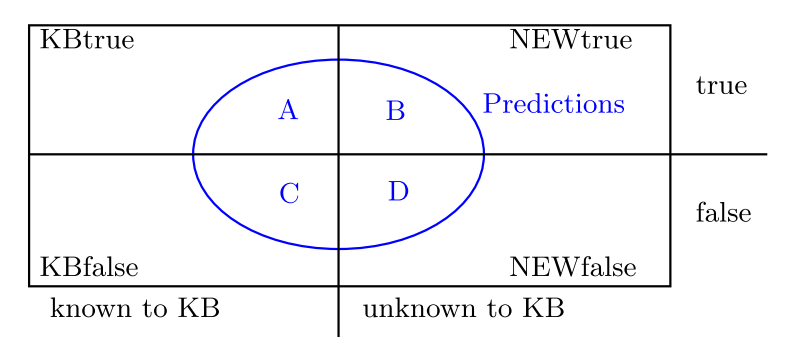
\includegraphics[width=\textwidth]{pui.png}
\caption{Prediction under Incompleteness.} \label{PCA}
\end{figure}

\begin{table}
\caption{Data size comparison of different datasets.}\label{datasetCom}
\centering
\begin{tabular}{|c|c|c|c|}
\hline
\textit{Dataset} & \textit{\#entities} & \textit{\#relations} & \textit{\#facts}\\
\hline
WN18RR & 40945 & 15 & 86835 \\
NELL-995 & 75492 & 200 & 154213 \\
FB15K-237 & 14504 & 237 & 272115 \\
WN18 & 40943 & 18 & 106088 \\
FB15K & 14951 & 1345 & 362538 \\
\hline
\textbf{Dbpeida} & \textbf{5900558} & \textbf{1322} & \textbf{18746174} \\
\hline
\end{tabular}
\end{table}

\subsection{Candidates Searching Components.}
Candidate searching is showed in Fig.(\ref{Newton_fig}).
\subsection{Reasons Displaying Components.}

\begin{enumerate}
  \item Eperiment 1:rule learning in a country and test in whole world
  \item Query test.
\end{enumerate}

\begin{figure}
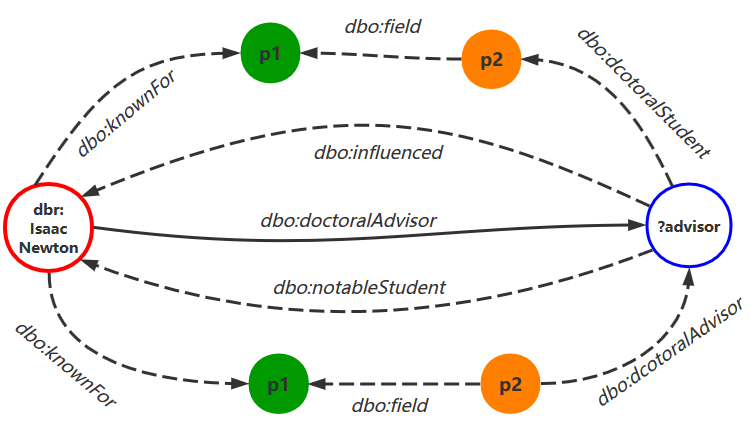
\includegraphics[width=\textwidth]{Newton.png}
\caption{Query Graph to get the advisors of Newton} \label{Newton_fig}
\end{figure}

\begin{figure}
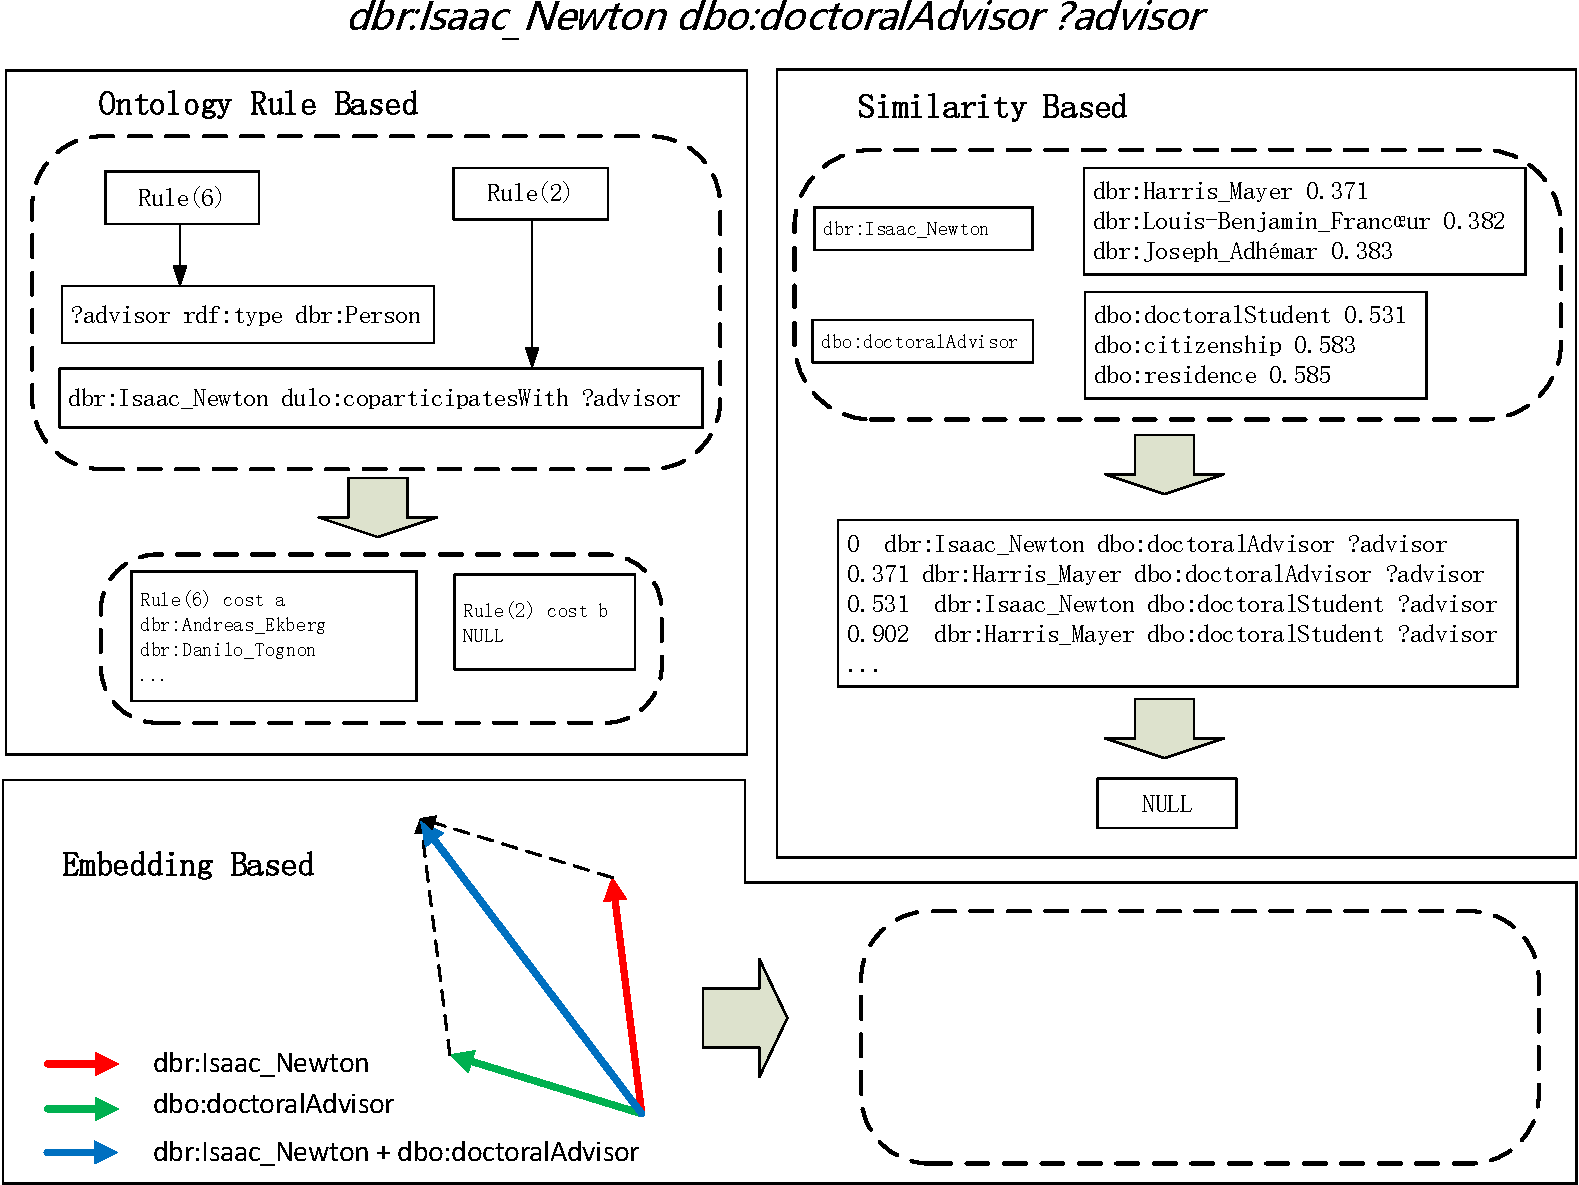
\includegraphics[width=\textwidth]{summary_three_cropped.pdf}
\caption{Summary of Three Baselines.} \label{summary_three}
\end{figure}

\bibliographystyle{splncs04}
\bibliography{xzlyu}
\end{document}

% \begin{table}
% \caption{Table captions should be placed above the
% tables.}\label{tab1}
% \begin{tabular}{|l|l|l|}
% \hline
% Heading level &  Example & Font size and style\\
% \hline
% Title (centered) &  {\Large\bfseries Lecture Notes} & 14 point, bold\\
% 1st-level heading &  {\large\bfseries 1 Introduction} & 12 point, bold\\
% 2nd-level heading & {\bfseries 2.1 Printing Area} & 10 point, bold\\
% 3rd-level heading & {\bfseries Run-in Heading in Bold.} Text follows & 10 point, bold\\
% 4th-level heading & {\itshape Lowest Level Heading.} Text follows & 10 point, italic\\
% \hline
% \end{tabular}
% \end{table}


% \noindent Displayed equations are centered and set on a separate
% line.
% \begin{equation}
% x + y = z
% \end{equation}
% Please try to avoid rasterized images for line-art diagrams and
% schemas. Whenever possible, use vector graphics instead (see
% Fig.~\ref{fig1}).



% \begin{theorem}
% This is a sample theorem. The run-in heading is set in bold, while
% the following text appears in italics. Definitions, lemmas,
% propositions, and corollaries are styled the same way.
% \end{theorem}
%
% the environments 'definition', 'lemma', 'proposition', 'corollary',
% 'remark', and 'example' are defined in the LLNCS documentclass as well.
%
% \begin{proof}
% Proofs, examples, and remarks have the initial word in italics,
% while the following text appears in normal font.
% \end{proof}
% For citations of references, we prefer the use of square brackets
% and consecutive numbers. Citations using labels or the author/year
% convention are also acceptable. The following bibliography provides
% a sample reference list with entries for journal
% articles~\cite{ref_article1}, an LNCS chapter~\cite{ref_lncs1}, a
% book~\cite{ref_book1}, proceedings without editors~\cite{ref_proc1},
% and a homepage~\cite{ref_url1}. Multiple citations are grouped
% \cite{ref_article1,ref_lncs1,ref_book1},
% \cite{ref_article1,ref_book1,ref_proc1,ref_url1}.
%
% ---- Bibliography ----
%
% BibTeX users should specify bibliography style 'splncs04'.
% References will then be sorted and formatted in the correct style.
%
